\section{Oxide}
\begin{frame}
\tableofcontents[currentsection]
\end{frame}

\begin{frame}
\frametitle{Esperimento ossido}
\begin{columns}
\begin{column}{0.5 \textwidth}
Abbiamo testato il risolutore lineare in due differenti situazioni, confrontate entrambe con sdevice. 

Per prima vediamo il caso $L_{contatto} = L_{lato}$
\end{column}
\begin{column}{0.5 \textwidth}
\begin{center}
\begin{figure}[!h]
          {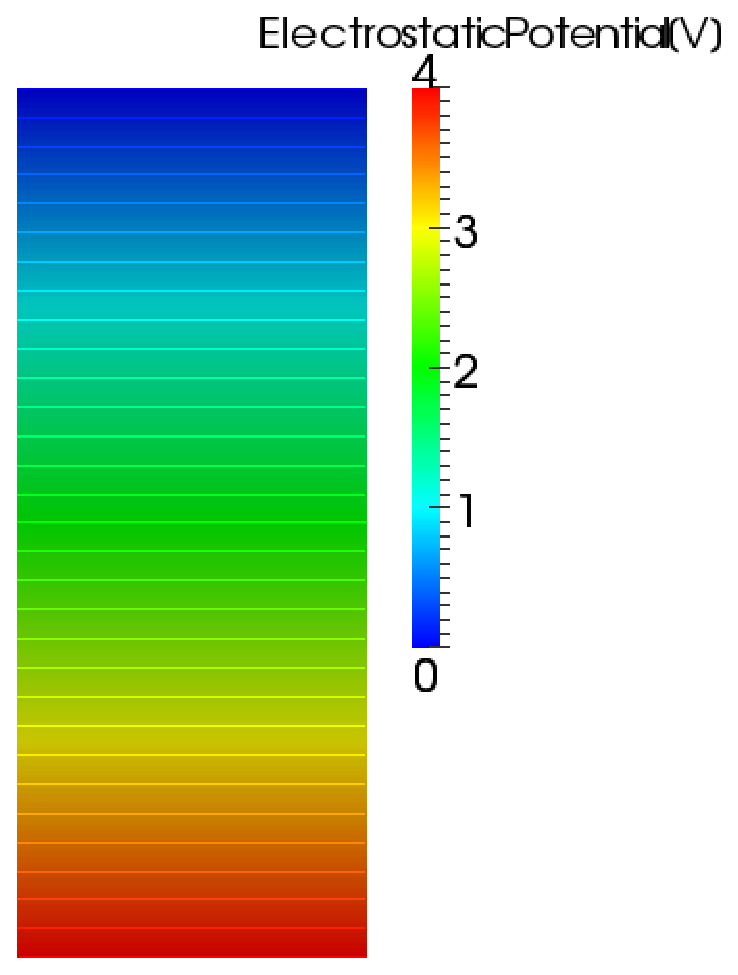
\includegraphics[scale=0.3]{ossidolineare}}
          \end{figure}
\end{center}
\end{column}

\end{columns}


\end{frame}

\begin{frame}
\frametitle{Esperimento ossido}
Di seguito il caso $L_{contatto} < L_{lato}$, soluzione non lineare

\begin{columns}

\begin{column}{0.3 \textwidth}
\begin{center}
\begin{figure}[!h]
          {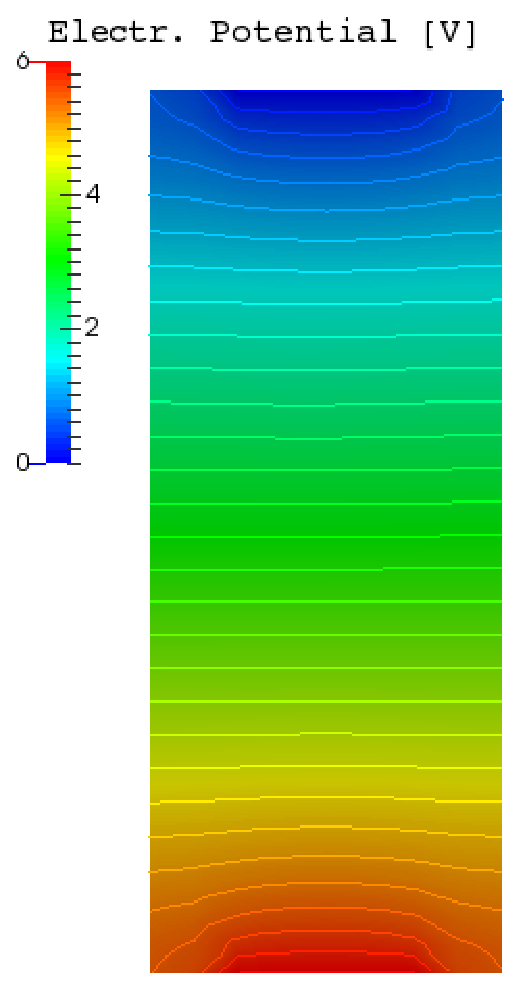
\includegraphics[scale=0.3]{potential}}
          \end{figure}
\end{center}
\end{column}

\begin{column}{0.3 \textwidth}
\begin{center}
\begin{figure}[!h]
          {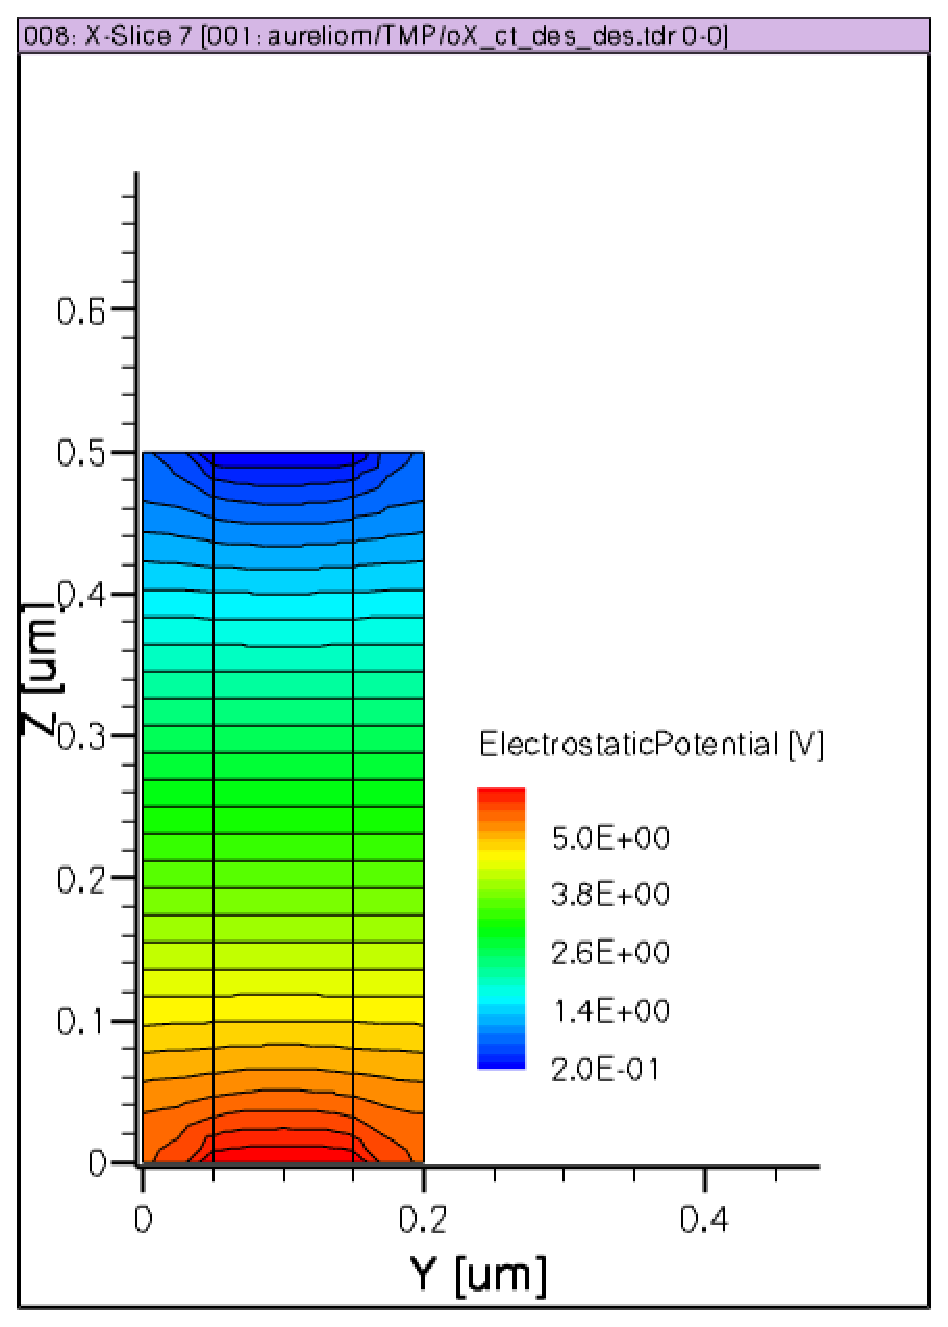
\includegraphics[scale=0.3]{ossido}}
          \end{figure}
\end{center}
\end{column}

\end{columns}

\end{frame}

